
%(BEGIN_QUESTION)
% Copyright 2011, Tony R. Kuphaldt, released under the Creative Commons Attribution License (v 1.0)
% This means you may do almost anything with this work of mine, so long as you give me proper credit

Gas flow control processes differ somewhat from liquid flow control processes, the former tending to be more difficult to control than the latter.  Consider the following process, controlling the flow of gas out of a pressure-controlled vessel:

$$\includegraphics[width=15.5cm]{i03400x01.eps}$$

When the flow indicating controller (FIC) is placed in manual mode and the output ``bumped'' 10\%, the result is certainly not what you would expect to see in a liquid flow control system:

$$\includegraphics[width=15.5cm]{i03400x02.eps}$$

Explain the odd shape of the process variable (PV) trend following the output step-change: why the flow increases, then ``sags,'' then stabilizes.  Identify a diagnostic test you could perform on this process to positively identify the source of this strange behavior, explaining how the result(s) of this next test would help you identify the cause.

\underbar{file i03400}
%(END_QUESTION)





%(BEGIN_ANSWER)

This is an example of a process with {\it interacting} control loops!

%(END_ANSWER)





%(BEGIN_NOTES)

One could try placing the pressure controller in manual mode as well to see if this alters the flow loop's response.  If so, then we know the PIC played a role in the strange response.  If not, then something in the flow loop is to blame.

Another test we could do is monitor the vessel pressure to see if it changes significantly during the flow open-loop test.  If so, we have reason to believe the PIC loop is the source of the weird droop.  If not, we should probably look toward the flow loop instrumentation as the source of the trouble (or see if there are any other interacting loops in the process we don't see on this diagram!).

%INDEX% Basics, control loop troubleshooting: determining cause of control problem
%INDEX% Control, PID tuning: interactive loops
%INDEX% Process: gas receiver flow control (generic)

%(END_NOTES)


